\appendix
%
% ***
\chapter{Programmcode Python}
% ***
%

	% ***
	\section{LIF-Modell}
	\label{sec:lifpy}
	% ***
	%\lstinputlisting[language=Python, firstline=23, lastline=38]{../Python/animation_lif/lif.py}

%
% ***
\chapter{Datenblatt Programm: TW-Circuit}
% ***
%

\begin{minipage}[t]{0.65\textwidth}
	\begin{mybox}{Name}
		\texttt{TW Circuit}
	\end{mybox}
	\begin{mybox}{Kurzinfo}
		\texttt{Lorem Ipsum Dolor sit amen.}
	\end{mybox}
	\begin{mybox}{Dependencies}
		\begin{itemize}
			\item \texttt{NumPy} aus dem \texttt{SciPy}-Package
			\subitem Numerische Berechnungen und Matrixoperationen.
			\item \texttt{matplotlib} aus dem \texttt{SciPy}-Package
			\subitem Plots und Grafiken anzeigen und exportieren.
			\item OpenAI Gym
			\subitem Simulationsumgebung \texttt{CartPole\_v0}
			\item \texttt{hickle}
			\subitem Performantes Speichern im HDF5-Format
			\item \texttt{os, time, datetime}
		\end{itemize}
	\end{mybox}
\end{minipage}
\hfill
\begin{minipage}[t]{0.35\textwidth}
	\begin{mybox}{QR-Code}
		\includegraphics[width=\textwidth]{figures/appendix/qr-code.pdf}
	\end{mybox}
	\begin{mybox}{Dateibaum}
		\vspace{0.3cm}
		\begin{forest}
			pic dir tree,
			where level=0{}{% folder icons by default; override using file for file icons
				directory,
			},
			[TW Circuit
			[docs]
			[information]
			[modules
			[inspect.py, file]
			[lif.py, file]
			[parameters.py, file]
			[random\_search\_v2.py, file]
			[visiualize.py, file]
			[weights.py, file]]
			[parameter\_dumps]
			[weight\_dumps]
			[main.py, file]]
		\end{forest}
	\end{mybox}
\end{minipage}


%
% ***
\chapter{Parameter mit guten Simulationsergebnissen}
% ***
%
	Nachfolgend werden verschiedene Simulationsläufe mit guten Ergebnissen im Detail vorgestellt. Dabei wird besonders auf die Parameter und Gewichte des neuronalen Netzes wert gelegt, da diese durch Simulationen gefunden wurden.\\
	Folgende Konvention wird eingehalten, um die Ergebnisse anschaulich darzustellen:\\
	Parameter der Nervenzellen:
	\begin{align}
		\boldsymbol{C_m} &= \begin{pmatrix}C_{AVA} & C_{AVD} & C_{PVC} & C_{AVB}\end{pmatrix},\\
		\boldsymbol{G_{Leak}} &= \begin{pmatrix}G_{AVA} & G_{AVD} & G_{PVC} & G_{AVB}\end{pmatrix},\\
		\boldsymbol{U_{Leak}} &= \begin{pmatrix}U_{AVA} & U_{AVD} & U_{PVC} & U_{AVB}\end{pmatrix}.
	\end{align}
	Parameter der Synapsen und Gap-Junctions:
	\begin{align}
		\boldsymbol{\sigma} &= \begin{pmatrix}\sigma_1 & \dots & \sigma_{16}\end{pmatrix},\\
		\boldsymbol{w} &= \begin{pmatrix}w_1 & \dots & w_{16}\end{pmatrix},\\
		\boldsymbol{\hat{w}} &= \begin{pmatrix}\hat{w}_1 & \hat{w}_{2}\end{pmatrix}.
	\end{align}
	Gewichte der Synapsen und Gap-Junctions:
	\begin{align}
		\boldsymbol{g} &= \begin{pmatrix}g_1 & \dots & g_{18}\end{pmatrix}.
	\end{align}
	Weitere Parameter und Einheiten sind der Tabelle \ref{label} zu entnehmen.
	\begin{figure}[!h] %[!t] ...
		\centering
		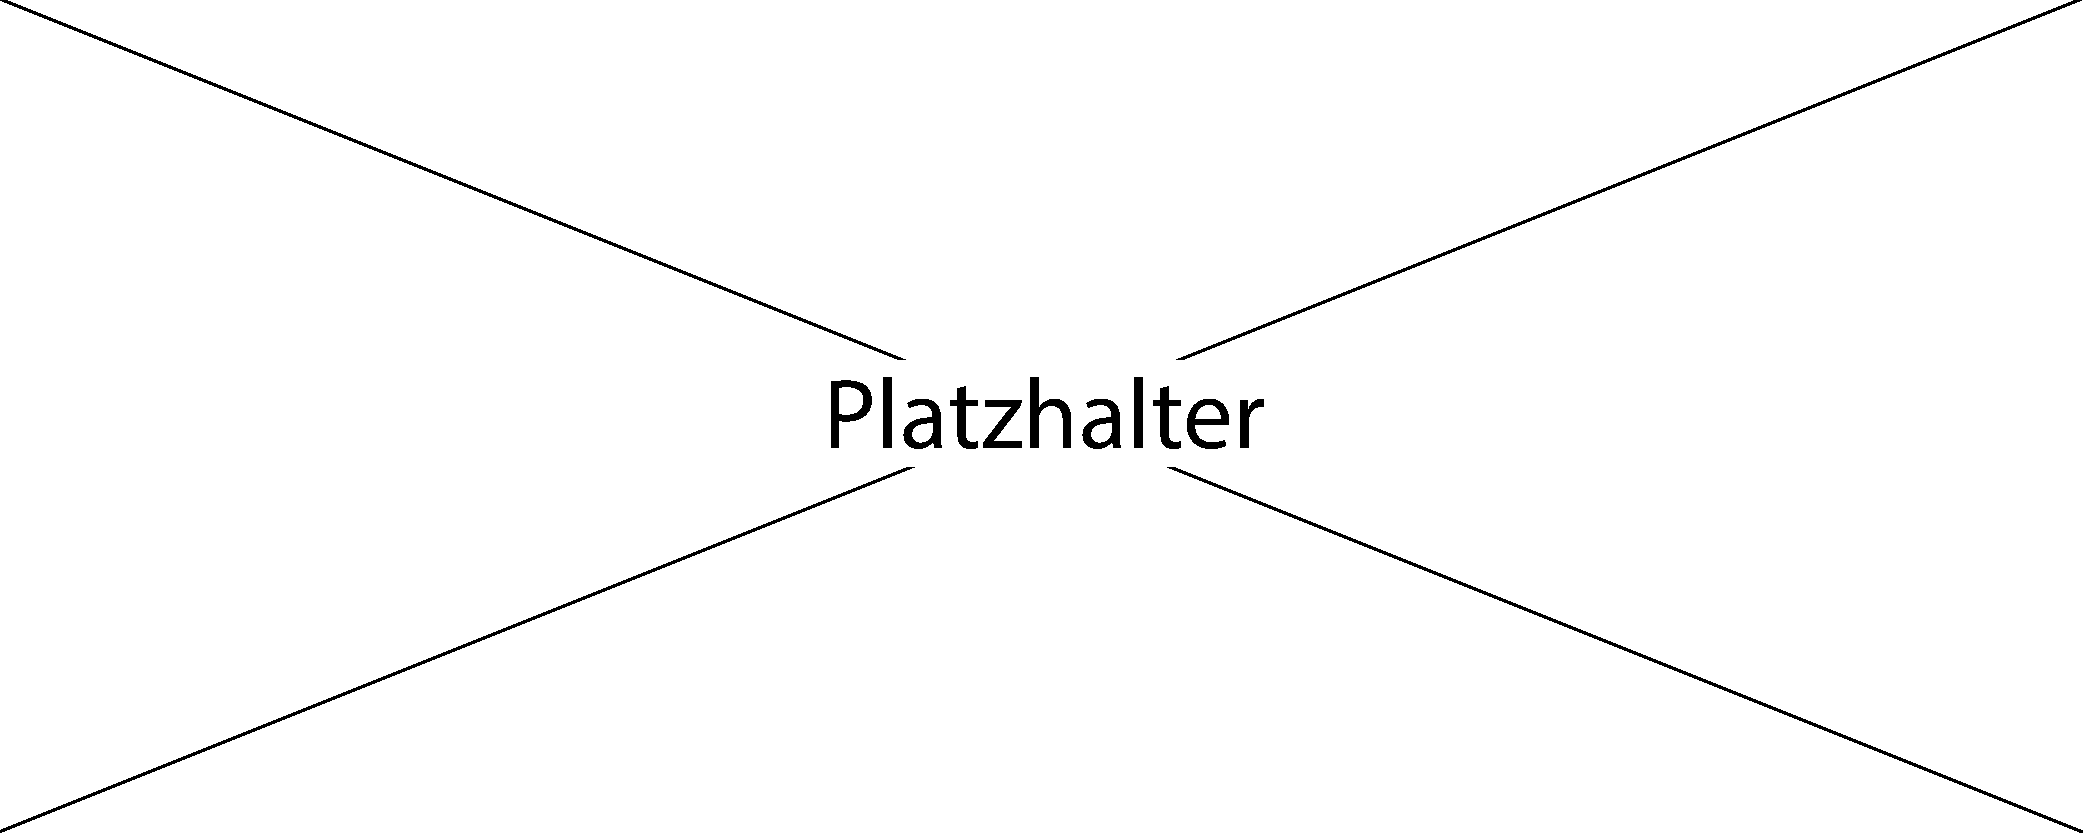
\includegraphics[width=12cm]{figures/sonstiges/platzhalter.pdf}
		\caption{Neuronales Netz mit Legende für Gewichte}
		\label{fig:erg_rs_flow}
	\end{figure}

	\afterpage{%
		\clearpage% Flush earlier floats (otherwise order might not be correct)
		\thispagestyle{empty}% empty page style (?)
		\begin{landscape}% Landscape page
			\centering % Center table
			\begin{tabular}{c@{\hskip 0.5cm}c@{\hskip 0.5cm}c@{\hskip 0.5cm}c@{\hskip 0.5cm}p{85mm}}    \toprule
				\setlength{\tabcolsep}{50pt}
				\renewcommand{\arraystretch}{1.5}
				\emph{Zeitstempel} 		& \emph{Algorithmus}		& \emph{Reward}	& \emph{Simulation (Dauer, Anz.)} 	& \emph{Parameter}		 \\\midrule
				
				20180817\_01-56-01		& RandomSearch - Parameter	& 131			& 12h, ca. 1 Mio. Simulationen		& Parameter der Nervenzellen \newline
				$\boldsymbol{C_m} = \begin{pmatrix}C_{AVA}, C_{AVD}, C_{PVC}, C_{AVB}\end{pmatrix}$,\newline
				$\boldsymbol{G_{Leak}} = \begin{pmatrix}G_{AVA}, G_{AVD}, G_{PVC}, G_{AVB}\end{pmatrix}$,\newline
				$\boldsymbol{U_{Leak}} = \begin{pmatrix}U_{AVA}, U_{AVD}, U_{PVC}, U_{AVB}\end{pmatrix}.$ \vspace{0.2cm} \newline
				Parameter der Synapsen \& GJ \newline
				$\boldsymbol{\sigma} = \begin{pmatrix}\sigma_1, \dots, \sigma_{16}\end{pmatrix}$,\newline
				$\boldsymbol{w} = \begin{pmatrix}w_1, \dots, w_{16}\end{pmatrix}$,\newline
				$\boldsymbol{\hat{w}} = \begin{pmatrix}\hat{w}_1, \hat{w}_{2}\end{pmatrix}$.\vspace{0.5cm}\\
				
				20180817\_13-56-01		& Weights - Gewichte		& 200			& 12h, ca. 400.000 Simulationen		& Gewichte der Synapsen \newline
				$\boldsymbol{g} = \begin{pmatrix}g_{1}, \dots, g_{18}\end{pmatrix}$.\\
				
				\bottomrule
				\hline
			\end{tabular}
			\captionof{table}{Table caption}% Add 'table' caption
		\end{landscape}
		\clearpage% Flush page
	}
	


%%% Local Variables: 
%%% mode: latex
%%% TeX-master: "main"
%%% End: 
